%=====================================================================
\section{Halo Finding and Particle Unbinding}\label{chap:phew}
%=====================================================================

Halo finding plays a central role in the exploitation of N-body
simulations. Paradoxically, a unique definition of what is a halo or a
sub-halo has never been adopted so far.  The current state of affairs
in the halo finding business is quite the opposite, with a multitude
of definitions emerging over the last decades, each definition
corresponding to a different halo finding algorithm.  The Halo Finder
Comparison Project \citep{MAD} lists 29 different codes and roughly
divides them into two distinct groups:
\begin{enumerate}
\item Percolation algorithms, for which particles are linked together
  if closer to each other than some specified linking length. The
  typical example is the algorithm ``\emph{friends-of-friends}''
  (thereafter FOF) \citep{FOF}.
\item Segmentation algorithms, for which space is segmented into
  separate regions around local peaks of the density field. Particles
  within these regions are then collected and assigned to the same
  halo or sub-halo. The typical example is the ``\emph{Spherical
  Overdensity}'' method (thereafter SOD) \citep{SO}.
\end{enumerate}
The outer boundary of the haloes are defined in both method by a
density iso-surface, whose exact value determines the properties of
the resulting halo statistics.  Halo catalogues derived from FOF and
SOD and their corresponding merger trees have been studied quite
extensively in the literature \citep[see e.g.][]{SUSSING_HALOFINDER}.

\subsection{The PHEW halo finder}

In this paper, we extend these earlier studies to the \phew\ halo
finder \citep{PHEW} developed specifically for the \ramses\ code
\citep{ramses}.  The \phew\ algorithm belongs to the category of
segmentation methods.  Particle masses are first deposited to the AMR
grid using the ``\emph{cloud-in-cell}'' technique. All density maxima
are then marked as potential sites for a \emph{clump}. Clumps are what
we call any structure, haloes and sub-haloes, in contexts where we
don't need to differentiate between them. The volume is then segmented
into peak patches by assigning each cell of the grid to the closest
density maximum in the direction of the steepest density gradient.

This segmentation method provides well defined regions separated by
density saddle surfaces. The minimum density in the saddle surface
between two adjacent peaks marks the saddle point between the two
peaks.  This well known method is often called `\emph{watershed
segmentation}`. In order to define proper halo boundaries, \phew\ uses
an outer density isosurface, like most methods described
above. Subhaloes, on the other hand, are just the ensemble of all
peak patches within the halo boundaries. This allows to identify
haloes and sub-haloes without the assumption of spherical symmetry,
unlike other popular methods such as SOD.

Subhaloes can be organised into a hierarchy of sub-structures based
on the same steepest gradient technique, for which individual clumps
can be assigned to the closest densest peak.  After this first pass,
only a few sub-haloes survived the merging process, which is then
repeated a second time, assigning these surviving sub-haloes to their
densest neighbours.  Ultimately, all sub-haloes will be collected into
a single peak that corresponds to the main halo. Each pass defines a
level in the hierarchy of sub-haloes. More details can be found in the
original \phew\ paper \citep{PHEW}.  As a consequence, a halo can have
a number of sub-haloes, each one of them containing subsub-haloes and
so on.  This well defined hierarchy is a very important feature for us
to uniquely assign particles to haloes and sub-haloes based on a
binding energy criterion.
 
There are four parameters that \phew\ requires a user to choose in
order to identify clumps and haloes.  Firstly, a ``relevance
threshold'' needs to be defined.  If for any given peak patch the
ratio of the peak's density to the maximal density of the entire
saddle surface of the respective peak patch is smaller than the chosen
relevance threshold, then the peak patch is considered to be noise,
not a genuine structure.  The peak patch is then merged into a
neighbour.  Secondly, a density threshold determines the minimal
density a cell needs to have to be part of any peak patch.  Thirdly, a
``saddle threshold'' defines the maximal density for a saddle surface
between two peak patches for the two patches to be considered parts of
two different haloes.  If the saddle surface density is above the
threshold, then the peak patches will be parts of the same halo (but
different sub-haloes within the host halo).  Finally, a mass threshold
determines the minimal mass a peak patch needs to have to be kept.  We
list the parameters that we used throughout this paper in Table~\ref{tab:phew-parameters}.

\begin{table}
\centering
\caption{Parameters used for the \phew\ clump finder throughout this
  paper.  The numerical values given can be directly used in the
  namelist file that \ramses\ uses to read in runtime parameters.
  Here $\bar \rho$ here is the mean background density and $m_p$ is
  the particle mass.}
\label{tab:phew-parameters}
\begin{tabular}[c]{l l l}
  parameter				&	value		& units \\
  \hline
  relevance threshold			&	3		& 1		\\
  density threshold			& 80			& $\bar \rho$ 	\\
  saddle threshold			& 200			& $\bar \rho$	\\
  mass threshold			& 10			& $m_p$		\\
  \hline
\end{tabular}
\end{table}
 
%Structure identified in this manner needs to be checked for being true condensations as opposed to arising from Poisson noise.	
%Such ``\emph{noise}'' peak patches are detected by computing the ratio of the density of each peak to the highest density of any cell of the peak patch that borders on another peak patch.
%If the ratio is sufficiently low, the patch is deemed to be noise and merged into the peak patch with whom it shares the aforementioned cell on its border with the highest density.
%Once the noise is identified and removed, the remaining structure consists only of peak patches, essentially clumps of particles, which satisfy the relevance condition. 
%These clumps represent the structure on the lowest scale.
%A large halo for example, which can very roughly be described as ``a large clump'' in a first approximation, would be decomposed into many small clumps at this point.
%The low level structure needs to be merged into composite clumps to form large scale haloes. 
%This merging is done iteratively and in doing so the hierarchy of substructure is established.
%A consequence, however, is that by construction, substructure will always have at least one neighbouring parent structure, which will have influence on the definition of when a particle is bound to the substructure.
	
%==========================================================
%\subsection{Particle Unbinding}\label{chap:unbinding}
%==========================================================

\subsection{Particle unbinding}

We now describe how we assign each dark matter particle to a given
sub-halo, a process that has not been implemented so far in the
\phew\ code.  For this, we follow a physically motivated criterion,
quite common in the halo finding literature, based on the binding
energy of the particle \citep[e.g.][]{AHF, subfind, skid}.  If a
particle is not bound to the first sub-halo of the hierarchy, it is
then passed recursively to the next sub-halo in the hierarchy, where
the binding energy is checked again and so on.  If the particle is not
bound to any sub-halo, it is assigned to the main halo.

In the previous hierarchical unbinding process, the key component is
the criterion adopted for deciding whether a particle is bound to a
sub-halo or not.  Traditionally, this is done using the {\it static}
gravitational potential, since we are dealing with a single time step
and we have to assume that the N-body system is stationary.  In this
case, a particle at position ${\bf r}$ is considered as unbound if its
velocity ${\bf v}$ exceeds the escape velocity given by
\begin{equation}
v_{\rm esc} = \sqrt{- 2\Phi(\mathbf{r})} 
\label{eq:boundv}
\end{equation}
More precisely, this means that the particle will be able to travel to
infinity where the potential goes to  zero. If the velocity is smaller
than the escape  velocity, the particle will follow a  bound orbit and
come back to its current location.  Note that this orbit can leave the
boundaries of the  sub-halo.  The particle will stay for  some time in
the sub-halo,  but can visit at  a later time a  neighbouring sub-halo
and then come back along the  same bound orbit.  This kind of particle
does not {\it exclusively} belong  to its original sub-halo. It should
be in fact assigned to the parent sub-halo in the hierarchy.  In order
to identify particles as more  strictly bound, we re-define the escape
velocity using the potential of the closest saddle point $\Phi_S$.
\begin{equation}
v_{\rm esc} = \sqrt{- 2(\Phi(\mathbf{r})-\Phi_S)} 
\label{eq:boundv_corr}
\end{equation}
This new  escape velocity is  smaller than the previous  one, allowing
more particle to  exceed it and leak out of  the current sub-halo into
neighbouring ones.  In what  follows, we will  use these two unbinding
criteria, calling the first method the ``loosely bound'' criterion and
calling   the   second   one   the   ``strictly   bound''   criterion.
Figure~\ref{fig:potentials} illustrates  the difference  between these
two  criteria.   The  gravitational  potential  of   two  neighbouring
sub-haloes labelled A  and B is represented.  We show  an example of a
strictly bound particle in each sub-halo,  and an example of a loosely
bound particle that can wander from one sub-halo to the other one.  If
one uses the first binding criterion, this loosely bound particle
will be  assigned to sub-halo A,  because this is where  it is located at
the present time.  If one uses the second, stricter binding criterion,
then the loosely bound particle will be assigned to the parent halo, but
not to sub-halo A nor B.


%A typical definition of a 'bound particle' can be obtained by considering an isolated clump in a time-independent scenario, where energy is conserved, a particle $i$ is considered to be bound if its velocity is smaller than the escape velocity:
%\begin{equation}
%	v_i < \sqrt{- 2 \cdot \Phi(\mathbf{r}_i)}  \quad \Leftrightarrow \quad \text{ particle is bound }\label{eq:boundv}
%\end{equation}

%where $\Phi$ is the gravitational potential, $\mathbf{r}_i$ is the particle's position and $v_i = ||\mathbf{v}_i||$ is the magnitude of the particle's velocity of each particle $i$, both given in the frame of reference of the centre of mass of the clump.
%An approximation for the potential $\Phi$ can be found by assuming spherical symmetry and solving the Poisson equation in the centre of mass frame of the clump.
%\begin{equation}
%	\Delta \Phi = \frac{1}{r^2}\frac{\del}{\del r} \left(r^2 \frac{\del}{\del r} \Phi \right) = 4 \pi G \rho
%\end{equation}



%One problem with condition \ref{eq:boundv} is that it assumes that clumps will be isolated, which by construction of the clump finder \phew\ sub-haloes will never be.
%The issues that arise from this fact can be understood by considering the boundaries of a particle's trajectory.
%These boundaries in a given potential $\Phi$ can be estimated using the conservation of energy:
%
%\begin{align}
%	E/m_p = \frac{1}{2} v^2 + \Phi = const.
%\end{align}
%

\begin{figure}
  \centering
  \fbox{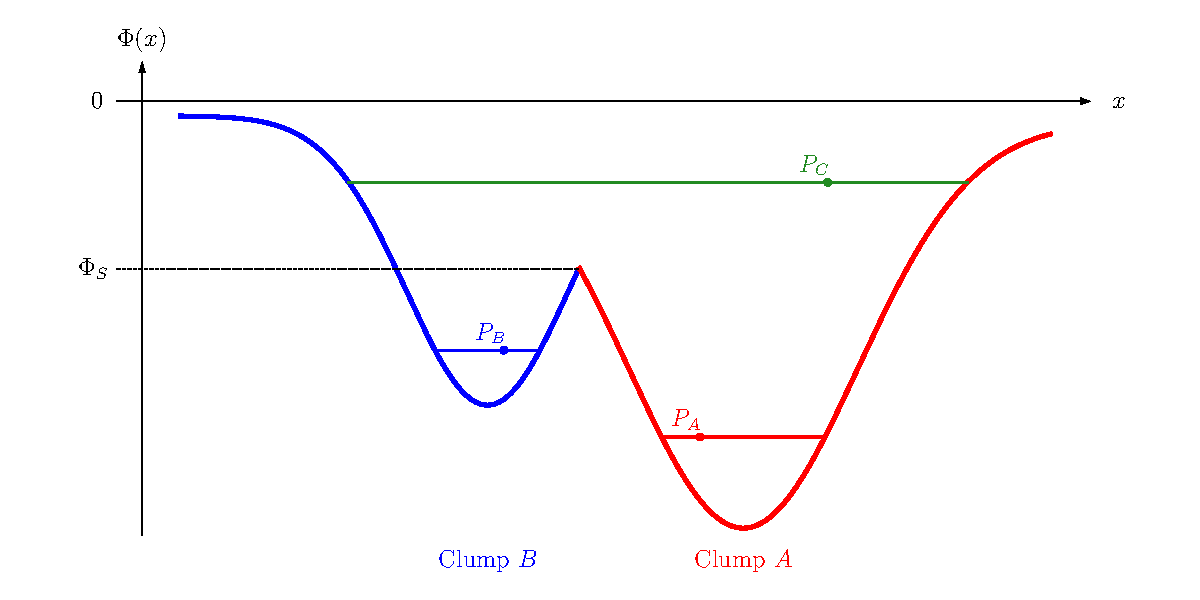
\includegraphics[width=.95\linewidth, keepaspectratio]{images/potentials_new.pdf}}%
  \caption{Simple sketch of the gravitational potential of a halo that
    consists of two clumps, $A$ and $B$.  The position of the
    horizontal lines marks the energies of three example particles,
    $P_A$, $P_B$, and $P_C$, while the length of the lines shows the
    spatial extent of the orbits.  We call particles like $P_A$ and
    $P_B$ ``strictly bound'', as their predicted orbit boundaries
    don't allow them to escape from the clump they are assigned to.
    Particle $P_C$ however, although energetically bound to clump $A$,
    can wander off deep into clump $B$, and for that reason is called
    ``loosely bound''. To discriminate between these two types of
    particles, we use the potential of the saddle point between clump
    $A$ and $B$ marked as $\Phi_S$.
  }%
  \label{fig:potentials}
  %	\endminipage\hspace*{\fill} 
\end{figure}
%
%Consider an isolated halo that consists of two clumps, $A$ and $B$, where $B$ is a smaller clump nested within clump $A$.
%Their potentials are qualitatively depicted in Figure \ref{fig:potentials}.
%The total energy per particle mass $E/m_p$ of the particle on the graph is the difference between the plotted norm of the potential and the kinetic energy on the $y$-axis.
%Because $v^2\geq 0$, the spatial boundaries of a particle's trajectory can be found by following the curve of allowed kinetic energies of the particle to the points where $v^2 = 0$.
%The marked particle $P$, even though initially assigned to clump $B$ and considered bound by condition \ref{eq:boundv}, is energetically allowed to leave the boundaries of clump $B$ and wander off deep into the neighbouring clump $A$.
%Should that occur in between two consecutive snapshots, then the particle $P$ will be rightfully found to belong to clump $A$ in the following snapshot.
%As such, the particle $P$ shouldn't be considered strictly bound to clump $B$.



%Three particles assigned to $B$ with different kinetic energies are marked, representing three different cases:
%%
%\begin{itemize}
%	\item Particle $\alpha$ has a kinetic energy higher than the potential, it is clearly not bound to the clump $B$.
%	\item Particle $\beta$ has a kinetic energy lower than the potential at that distance from the centre of mass, so it will remain bound on an elliptic trajectory around the centre of mass.
%	\item Particle $\gamma$ is considered energetically bound to the clump just like $\beta$, i.e. it satisfies condition \eqref{eq:boundv}, but it won't necessarily remain on an elliptic trajectory around clump $B$'s centre of mass: Because of clump $A$'s neighbouring potential, the particle can leave the boundaries of clump $B$ and wander off deep into clump $A$.
%\end{itemize}
%%

%To address this occurrence the condition for a particle to be bound needs to be modified appropriately: its trajectory must never reach the common surface between any two clumps.
%Defining $\Phi_S$ to be the potential of clump $B$ at the interface to any neighbouring structure that is closest to $B$'s centre of mass, the condition for a particle to be bound \emph{exclusively} to a particular clump can be written as
%
%\begin{equation}
%	v < \sqrt{ - 2(\Phi - \Phi_S) } \label{eq:boundv_corr}
%\end{equation}


%We have verified that according to expectations, demanding particles to be exclusively bound, i.e. satisfying condition \ref{eq:boundv_corr}, will tend to find more unbound particles than not doing so, where particles close to the centre of mass are be more likely to be exclusively bound than the particles closer to the outer boundary of the sub-halo.

When computing the velocity of the particle, it is important to use
the velocity {\it relative} to the velocity of the sub-halo centre of
mass (also called the bulk velocity of the sub-halo).  Because of this
requirement, the unbinding process has to be performed iteratively,
since removing a particle that is unbound requires to recompute the
centre of mass velocity.  Let us finally repeat that the particle
unbinding is performed recursively, following the sub-halo hierarchy
from the bottom up.  Starting with the lowest (finest) level of
sub-haloes, unbound particles are assigned to the higher (coarser)
level of parent sub-halo for unbinding, and so on following the
structure hierarchy.  Particles that are unbound from all sub-haloes
are collected into the main halo, marking the end of the hierarchical
unbinding process.


